\label{Chapter:connection:triplets}
We have seen how the framework presented in \cite{oord_representation_2019} uses a generative approach as a part of the representation learning process. Let us set in the case of learning representations of images. In this case, generative models must \emph{generate} each pixel on the image. This can be extremely computationally expensive. 

Until now, we had been trying to minimize the loss in Equation \eqref{NCE:loss}, which we proved that maximizes a lower bound in the mutual information. However, some papers such as \cite{chen_simple_2020}, \cite{tschannen_mutual_2020}, suggest that it is unclear if the success of their methods is caused by the maximization of mutual information between the latent representations, or by the specific form that the constrastive loss has.

In fact, in \cite{tschannen_mutual_2020} they provide empirical proof for the loose connection between the success of the methods that use MI maximization and the utility of the MI maximization in practice. They also empirically proof  that the encoder architecture can be more important than the estimator used to determine the MI.

Even with the empirically proved disconnection between MI maximization and representation quality, recent works that have used the loss function \ref{NCE:loss} have obtained state-of-art results in practice. There is an explanation for this, connecting the recently mentioned loss with a popular triplet loss.

\section{From deep metric learning to triplet losses and its generalization}

Distance metric learning aims to learn an embedding representation of an input data $x$ that preserves the distance between similar data points close and also makes de distance between different datapoints far on the embedding space \citep{Sohn2016ImprovedDM}.

We will consider sets of triplets $(x,\ps,\ns)$ where:
\begin{itemize}
\item The element $x$ is an anchor point,
\item The element $\ps$ is a positive instance,
\item The element $\ns$ is a negative instance.
\end{itemize}

\begin{nexample}
    Let us present a very simple example. If our input image is a cat, that would be the anchor $x$. Clearly, a positive instance would be an image of another cat or even the same cat seen from another perspective. A negative instance would be a photo of any other animal, in this case we use a dog.
    \begin{figure}[H]%!htb]
        \minipage{0.32\textwidth}
          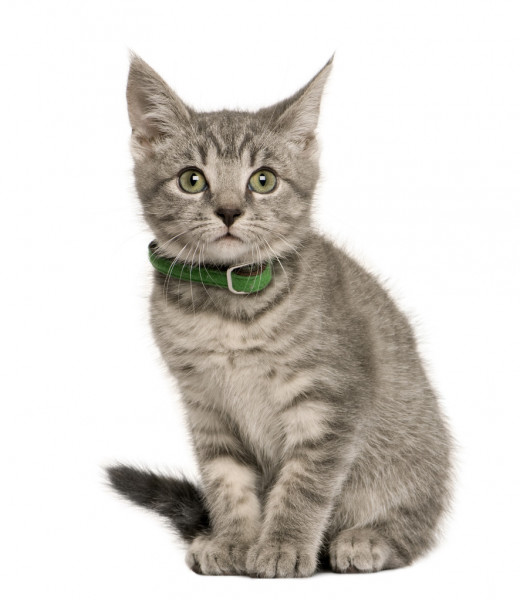
\includegraphics[width=\linewidth]{media/c1}
          \caption*{Anchor}\label{fig:cat1}
        \endminipage\hfill
        \minipage{0.32\textwidth}%
          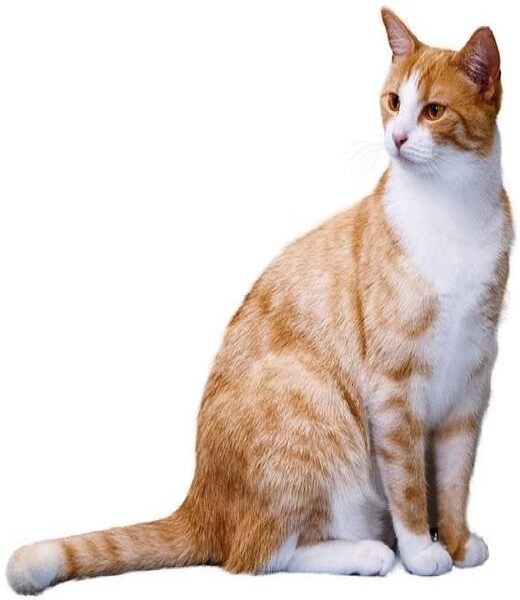
\includegraphics[width=\linewidth]{media/c2}
          \caption*{Positive example}\label{fig:c2}
        \endminipage
        \minipage{0.32\textwidth}%
          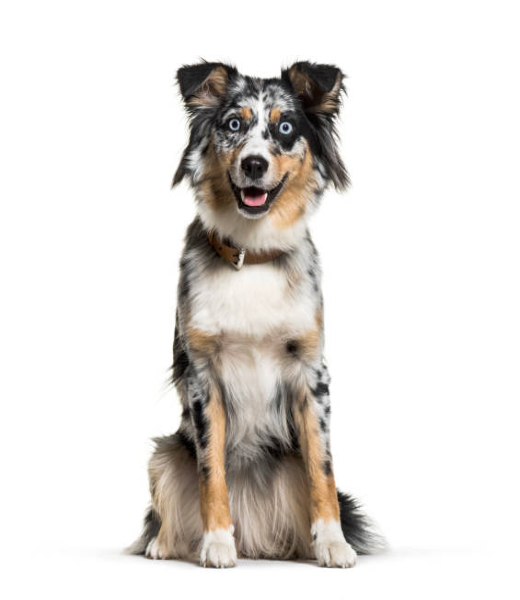
\includegraphics[width=\linewidth]{media/doggo}
          \caption*{Negative example}\label{fig:doggo}
        \endminipage
        \caption{Example of an anchor $x$, a positive instance $\ps$ and a negative instance $\ns$. Images obtained from \emph{Google}.}
        \end{figure}
    \end{nexample}
    


The main idea is to learn a representation of $x$, say $g(x)$, such that the distance of the representation of the input is closer in distance to the representation of the positive sample $\ps$ than the representation of the negative sample $\ns$. Using the norm\footnotemark, we can formally express that as follows: 
$$
\norm{g(x) - g(\ps)}_2 \leq \norm{g(x) - g(\ns)}_2,
$$
for each triplet in the set.


%------------- Footnotemark
\footnotetext{A definition of the norm can be found on Appendix \ref{APPENDIX:A}, Definition \ref{def:norm}. }
%----------------------


Support-vector machines (SVMs) are supervised learning models used for classification or regression problems. They are one of the most robust predicion methods. They search for a hyperplane $h$ in high or infinite dimensional space that separates the data as much as possible, making use of \emph{support vectors}, the datapoints that are closest to the hyperplane. If the data is linearly separable, we can select two hyperplanes $h_1,h_2$ that are parallel to $h$ and making the distance from them to $h$ as large as possible. That region is called the \emph{margin}.

Coming back to our triplets problem, we also want to introduce a margin between the distances of the elements of the triplets, in order to separate positive examples from negative examples as much as possible. This way, we introduce a \emph{margin} term $\alpha$, rewriting our last equation as follows:
\[
\norm{g(x) - g(\ps)}_2 + \alpha < \norm{g(x) - g(\ns)}_2.
\]
Using this inequality, we can define a hinge loss function for each triplet in the set:
\begin{equation}\label{triplet:single:loss}
\ell^\alpha (x,\ps,\ns) = \max \left(0, \norm{g(x) - g(\ps)}_2^2 - \norm{g(x) - g(\ns)}_2^2 + \alpha\right).
\end{equation}
This loss has been defined for a single triplet. Now, we can define a global loss that accumulates the loss in Equation \eqref{triplet:single:loss} using all the triplets in set.

\begin{ndef}
Given a set of triplets, each containing an anchor, a positive example and a negative example, $\mathcal T = \{(x_i,\ps_i,\ns_i)\}_{i \in \Lambda}$, we define a triplet loss as follows:
\begin{equation}\label{triplet:sum:loss}
\mathcal L (x_i,\ps_i,\ns_i) = \sum_{i \in \Lambda} \ell^\alpha(x_i,\ps_i,\ns_i).
\end{equation}

\end{ndef}



We use this loss to train models in order to improve the representations obtained.It would be interesting to present the model non-trivial metric to the learning algorithm. When the representation $g$ improves, this is harder to do, and this results in slow convergence and expensive data sampling methods.

\subsection*{Generalization of triplet losses}

In a single evaluation of the loss function over a triplet during the learning process, we are comparing one positive sample to one negative sample. In practice, after looping over sufficiently many triplets, we expect the distance between positive examples and negative examples to be maximized. However, this will surely be a slow process if our dataset has many examples and also, in each step we will be separating the positive element from the specific negative element to which we are comparing it in that evaluation. Thus, the technique might be unstable \citep{Sohn2016ImprovedDM}.

In order to fix this, a good idea would be to compare in each evaluation a positive sample with multiple negative samples, generalizing the case exposed before. This way, we would like the positive sample to increase its distance to \emph{all} of the negative samples at the same time. Let us present a loss that generalizes the loss in Equation \eqref{triplet:sum:loss}.

\begin{ndef}
Let $\ps$ be a positive example of the anchor $x$, and consider the set $X^- = \{\ns_1,\cdots,\ns_{N-1}\}$ of $(N-1)$ negative samples. Given an encoder $g$, the $(N+1)-$tuplet loss is defined as follows:
\begin{equation}\label{nplus1:tuplet:loss}
\mathcal L_{(N+1)-\text{tuplet}}(x,\ps,X^-) = \log \left( 1+ \sum_{i=1}^{N-1} \exp \left(g(x)^T g(\ns_i) - g(x)^T g(\ps)\right)\right) 
\end{equation}
\end{ndef}

\begin{remark}
If we consider the case $N=2$, we have
\[
\mathcal L_{(2+1)-\text{tuplet}}(x,\ps,\ns) = \log \left( 1+ \exp \left(g(x)^Tg(\ns) - g(x)^T g(\ps)\right)\right).
\]
This expression is very similar to the one in Equation \eqref{triplet:single:loss}. In fact, if the norm in Equation \eqref{triplet:single:loss} is unit, if $g$ minimizes $\mathcal L_{(2+1)-\text{tuplet}}$, then it minimizes $\ell^\alpha$, and hence both losses are equivalent.
\end{remark}

Applying the $(N+1)-$tuplet loss in deep metric learning is computationally expensive. Indeed, if we apply Stochastic Gradient Descent (SGD) with batch size $M$, then we have to evaluate $M \times (N+1)$ times our function $\ell^\alpha$ in each update. Because of this, if we increase $M$ and $N$, the number of evaluations grows quadratically. We would like to avoid this.

Consider the set of $N$ pairs of examples, with the constraint of each pair belonging to a different class, i.e. $X = \{(x_1,\ps_1),\cdots,(x_N,\ps_N)\}$ with $y_i \neq y_j$ for all $i \neq j$. We now build $N$ tuplets where each tuplet has all the positive samples and the $i-th$ anchor, that is:
\[
\{S_i\}_{i=1}^N, \quad \text{where} \quad S_i = \{x_i, \ps_1,\cdots,\ps_N\}.  
\]
We can consider that each tuplet has $x_i$ as anchor, $\ps_i$ as positive example and $\ps_j$ for $j \neq i$ as negative samples, since they were all from different classes.



The InfoNCE loss on Equation \eqref{NCE:loss} has proved to be useful in representation learning. Let us consider a reformulation on it. Firstly, since $f_k$ was an exponential, we can also consider $e^f$ and remove the exponential from $f$, this is just notation. Now, we can rewrite the InfoNCE objective as follows
\begin{align*}
I_{NCE}  & = E\left[ \frac{1}{N} \sum_{i = 1}^N \log \frac{e^{f(x_i,y_i)}}{\frac{1}{N}\sum_{j=1}^N e^{f(x_i,y_j)}}\right]\\
& = a\\
& = \log N - E\left[ \frac{1}{N} \sum_{i=1}^N \log \left( 1+ \sum_{j\neq i}e^{f(x_i,y_j)- f(x_i,y_i)}\right)\right]
\end{align*}

